\documentclass{beamer}
\usetheme{AnnArbor}
\usecolortheme{spruce}
\usepackage{circuitikz}
\usepackage{graphicx}

\title{Multiplexers \& Demultiplexers}
\subtitle{Convenience in circuit design}
\author[A Praveen \& A Krishnan]{Akilesh Praveen \& Ashwath Krishnan}
\institute{UMD}
\date{\today}



\begin{document}

    % title page
    \begin{frame}
        \titlepage
    \end{frame}
    
    % table of contents
    \begin{frame}
        \frametitle{Agenda}
        \tableofcontents
    \end{frame}
    
    \section{Announcements}
    
        \begin{frame}
                \vfill
                \centering
                \begin{beamercolorbox}[sep=8pt,center,shadow=true,rounded=true]{title}
                    \usebeamerfont{title}Announcements\par%
                \end{beamercolorbox}
                \vfill
             \end{frame}
    
        \subsection{Project 3}
        
            
            
            \begin{frame}
                \frametitle{Project 4}
                \begin{itemize}
                    \item Project 4's been released, and the name of the game is multipliers.
                    \item You'll find everything you need under the 'week 5' section on the course website
                    \item Today's lecture will give you background knowledge that will help you implement multiplexers and demultiplexers.
                    
                    \item More info to come at the end of lecture
                    
                \end{itemize}
            \end{frame}
            
    \section{Multiplexers \& Demultiplexers}
    
    	\subsection{Introduction}
    	
    	\begin{frame}
    		\frametitle{Multiplexers \& Demultiplexers}
    		
    		\begin{itemize}
    			\item A \textbf{Multiplexer} is often called a 'mux'.
    			\item A \textbf{Demultiplexer} is often called a 'demux'.
    		\end{itemize}
    		
		\end{frame}  
		
		\begin{frame}
    		\frametitle{Multiplexers \& Demultiplexers}
    		
    		\begin{itemize}
    			\item A \textbf{Multiplexer} is often called a 'mux'.
    			\item A \textbf{Demultiplexer} is often called a 'demux'.
    			\item The question is- what are they?
    		\end{itemize}
    		
		\end{frame}
		
		\begin{frame}
			\frametitle{Need necessitates solution}
			\begin{itemize}
				\item The need for \textbf{Multiplexers} arose due to the presence of a certain problem in digital circuit design.
				\item Remember our buses + encoders and decoders?
				\item It turns out, there are a lot of different circuits that would require us to have a fair amount of parallel wires.
				
			\end{itemize}
		\end{frame}		 
		
		\begin{frame}
			\frametitle{An example}
      


\tikzset{every picture/.style={line width=0.75pt}} %set default line width to 0.75pt        

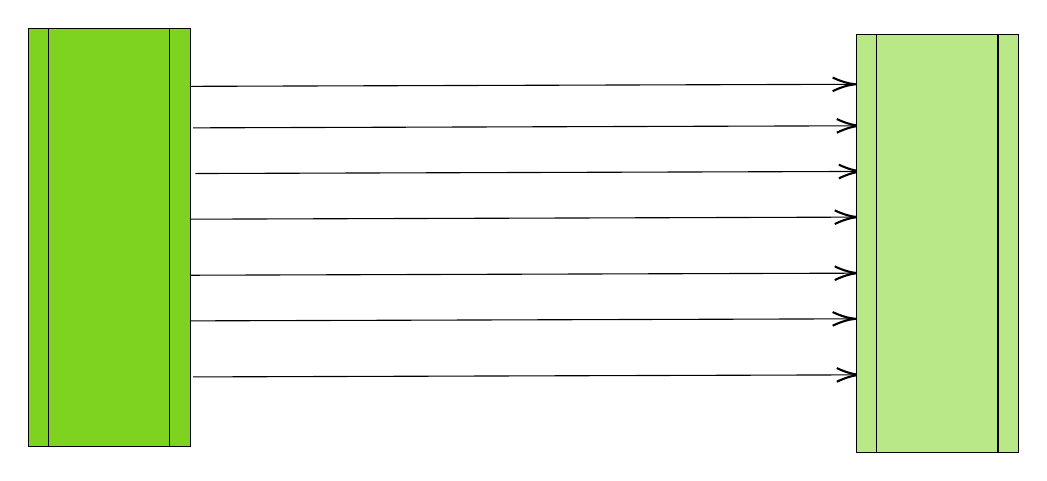
\begin{tikzpicture}[x=0.75pt,y=0.75pt,yscale=-1,xscale=1]
%uncomment if require: \path (0,300); %set diagram left start at 0, and has height of 300

%Straight Lines [id:da797417316267886] 
\draw    (98.5,64) -- (417.5,63.01) ;
\draw [shift={(419.5,63)}, rotate = 539.8199999999999] [color={rgb, 255:red, 0; green, 0; blue, 0 }  ][line width=0.75]    (10.93,-3.29) .. controls (6.95,-1.4) and (3.31,-0.3) .. (0,0) .. controls (3.31,0.3) and (6.95,1.4) .. (10.93,3.29)   ;
%Straight Lines [id:da9867161861578443] 
\draw    (100.5,84) -- (419.5,83.01) ;
\draw [shift={(421.5,83)}, rotate = 539.8199999999999] [color={rgb, 255:red, 0; green, 0; blue, 0 }  ][line width=0.75]    (10.93,-3.29) .. controls (6.95,-1.4) and (3.31,-0.3) .. (0,0) .. controls (3.31,0.3) and (6.95,1.4) .. (10.93,3.29)   ;
%Straight Lines [id:da17622714748979218] 
\draw    (101.5,106) -- (420.5,105.01) ;
\draw [shift={(422.5,105)}, rotate = 539.8199999999999] [color={rgb, 255:red, 0; green, 0; blue, 0 }  ][line width=0.75]    (10.93,-3.29) .. controls (6.95,-1.4) and (3.31,-0.3) .. (0,0) .. controls (3.31,0.3) and (6.95,1.4) .. (10.93,3.29)   ;
%Straight Lines [id:da3187699597458509] 
\draw    (99.5,128) -- (418.5,127.01) ;
\draw [shift={(420.5,127)}, rotate = 539.8199999999999] [color={rgb, 255:red, 0; green, 0; blue, 0 }  ][line width=0.75]    (10.93,-3.29) .. controls (6.95,-1.4) and (3.31,-0.3) .. (0,0) .. controls (3.31,0.3) and (6.95,1.4) .. (10.93,3.29)   ;
%Straight Lines [id:da5165041416753314] 
\draw    (99.5,155) -- (418.5,154.01) ;
\draw [shift={(420.5,154)}, rotate = 539.8199999999999] [color={rgb, 255:red, 0; green, 0; blue, 0 }  ][line width=0.75]    (10.93,-3.29) .. controls (6.95,-1.4) and (3.31,-0.3) .. (0,0) .. controls (3.31,0.3) and (6.95,1.4) .. (10.93,3.29)   ;
%Straight Lines [id:da10098087423079927] 
\draw    (98.5,177) -- (417.5,176.01) ;
\draw [shift={(419.5,176)}, rotate = 539.8199999999999] [color={rgb, 255:red, 0; green, 0; blue, 0 }  ][line width=0.75]    (10.93,-3.29) .. controls (6.95,-1.4) and (3.31,-0.3) .. (0,0) .. controls (3.31,0.3) and (6.95,1.4) .. (10.93,3.29)   ;
%Straight Lines [id:da14963118622609028] 
\draw    (100.5,204) -- (419.5,203.01) ;
\draw [shift={(421.5,203)}, rotate = 539.8199999999999] [color={rgb, 255:red, 0; green, 0; blue, 0 }  ][line width=0.75]    (10.93,-3.29) .. controls (6.95,-1.4) and (3.31,-0.3) .. (0,0) .. controls (3.31,0.3) and (6.95,1.4) .. (10.93,3.29)   ;
%Flowchart: Prodefined Process [id:dp12787585466953033] 
\draw  [fill={rgb, 255:red, 126; green, 211; blue, 33 }  ,fill opacity=1 ] (21,36) -- (99,36) -- (99,237.5) -- (21,237.5) -- cycle ; \draw   (30.75,36) -- (30.75,237.5) ; \draw   (89.25,36) -- (89.25,237.5) ;
%Flowchart: Prodefined Process [id:dp585559902263576] 
\draw  [fill={rgb, 255:red, 184; green, 233; blue, 134 }  ,fill opacity=1 ] (420,39) -- (498,39) -- (498,240.5) -- (420,240.5) -- cycle ; \draw   (429.75,39) -- (429.75,240.5) ; \draw   (488.25,39) -- (488.25,240.5) ;




\end{tikzpicture}


			\begin{itemize}
				\item We've started creating circuits that have a sizable amount of wires associated with them
				\item It turns out, extending \textbf{all} of these wires is pretty expensive and space-consuming, given just how many wires we have to build
			\end{itemize}
			
			
			

		\end{frame}	
		
		
		\begin{frame}
			\frametitle{Parallel Signals}
			\begin{itemize}
				\item This phenomenon is known as having many \textbf{parallel signals}.
				\item They use a ton of wires!
				\item I'm sure everyone is well aware of how much more effort it is to place one extra line of wires in Minecraft, which makes you wonder how much harder it is to do in real life
				\item If we're going to be extending these wires over long distances, are there more efficent ways to handle that many signals?
			\end{itemize}
		\end{frame}	
		
		\begin{frame}
			\frametitle{Parallel Signals}
			\begin{itemize}
				\item Yes!!!
				\item Your answer can be found in \textbf{Multiplexers} and \textbf{Demultiplexers}.
			\end{itemize}
		\end{frame}			  	        
        
    
    	\subsection{What are Muxes and Demuxes?}
    	
    	\begin{frame}
    		\frametitle{What are they?}
    		\begin{itemize}
    			\item A \textbf{Multiplexer}, or \textbf{Mux}, takes a bunch of parallel wires and condenses all of them down to a singular \texttt{OUT} wire and a few \texttt{SELECT} wires.
    			\item A \textbf{Demultiplexer}, or \textbf{Demux}, takes a singular \texttt{IN} wire and a few \texttt{SELECT} wires, and sends the \texttt{IN} signal down the appropriate output wire.
    		\end{itemize}
    	\end{frame}
    	
    	\begin{frame}
    		\frametitle{What are they?}
    		\begin{itemize}
    			\item A \textbf{Multiplexer}, or \textbf{Mux}, takes a bunch of parallel wires and condenses all of them down to a singular \texttt{OUT} wire and a few \texttt{SELECT} wires.
    			\item A \textbf{Demultiplexer}, or \textbf{Demux}, takes a singular \texttt{IN} wire and a few \texttt{SELECT} wires, and sends the \texttt{IN} signal down the appropriate output wire.
    		\end{itemize}
    		
    		
			

\tikzset{every picture/.style={line width=0.75pt}} %set default line width to 0.75pt        

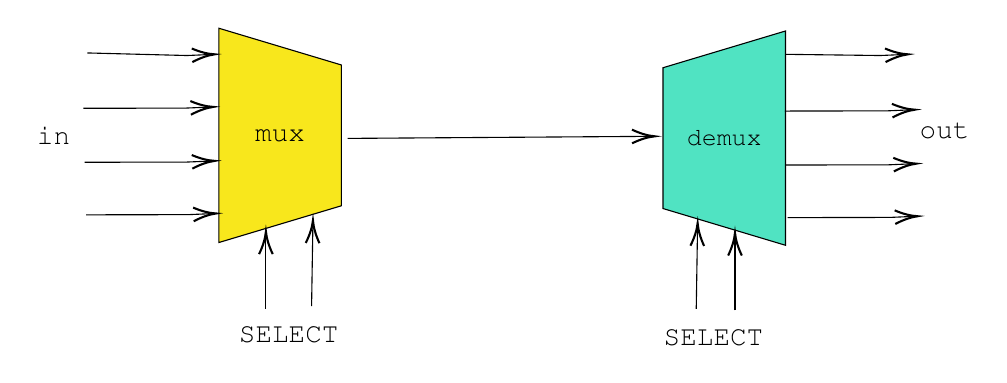
\begin{tikzpicture}[x=0.75pt,y=0.75pt,yscale=-1,xscale=1]
%uncomment if require: \path (0,300); %set diagram left start at 0, and has height of 300

%Shape: Trapezoid [id:dp9676716720394224] 
\draw  [fill={rgb, 255:red, 248; green, 231; blue, 28 }  ,fill opacity=1 ] (127,83.42) -- (186,101.12) -- (186,168.97) -- (127,186.67) -- cycle ;
%Shape: Trapezoid [id:dp8112150659093363] 
\draw  [fill={rgb, 255:red, 80; green, 227; blue, 194 }  ,fill opacity=1 ] (400,188) -- (341,170.3) -- (341,102.45) -- (400,84.75) -- cycle ;
%Straight Lines [id:da17513161874771777] 
\draw    (189,136.5) -- (335,135.51) ;
\draw [shift={(337,135.5)}, rotate = 539.61] [color={rgb, 255:red, 0; green, 0; blue, 0 }  ][line width=0.75]    (10.93,-3.29) .. controls (6.95,-1.4) and (3.31,-0.3) .. (0,0) .. controls (3.31,0.3) and (6.95,1.4) .. (10.93,3.29)   ;
%Straight Lines [id:da7314260725072124] 
\draw    (63.67,95.33) -- (111.64,96.57) -- (123,96.08) ;
\draw [shift={(125,96)}, rotate = 537.5699999999999] [color={rgb, 255:red, 0; green, 0; blue, 0 }  ][line width=0.75]    (10.93,-3.29) .. controls (6.95,-1.4) and (3.31,-0.3) .. (0,0) .. controls (3.31,0.3) and (6.95,1.4) .. (10.93,3.29)   ;
%Straight Lines [id:da32898600894177765] 
\draw    (61.67,122) -- (110.98,121.9) -- (122.34,121.42) ;
\draw [shift={(124.33,121.33)}, rotate = 537.5699999999999] [color={rgb, 255:red, 0; green, 0; blue, 0 }  ][line width=0.75]    (10.93,-3.29) .. controls (6.95,-1.4) and (3.31,-0.3) .. (0,0) .. controls (3.31,0.3) and (6.95,1.4) .. (10.93,3.29)   ;
%Straight Lines [id:da7983247275507934] 
\draw    (62.33,148) -- (111.64,147.9) -- (123,147.42) ;
\draw [shift={(125,147.33)}, rotate = 537.5699999999999] [color={rgb, 255:red, 0; green, 0; blue, 0 }  ][line width=0.75]    (10.93,-3.29) .. controls (6.95,-1.4) and (3.31,-0.3) .. (0,0) .. controls (3.31,0.3) and (6.95,1.4) .. (10.93,3.29)   ;
%Straight Lines [id:da04807653219902874] 
\draw    (63,173.33) -- (112.31,173.23) -- (123.67,172.75) ;
\draw [shift={(125.67,172.67)}, rotate = 537.5699999999999] [color={rgb, 255:red, 0; green, 0; blue, 0 }  ][line width=0.75]    (10.93,-3.29) .. controls (6.95,-1.4) and (3.31,-0.3) .. (0,0) .. controls (3.31,0.3) and (6.95,1.4) .. (10.93,3.29)   ;
%Straight Lines [id:da5159526044803394] 
\draw    (400.33,96) -- (445.64,96.57) -- (457,96.08) ;
\draw [shift={(459,96)}, rotate = 537.5699999999999] [color={rgb, 255:red, 0; green, 0; blue, 0 }  ][line width=0.75]    (10.93,-3.29) .. controls (6.95,-1.4) and (3.31,-0.3) .. (0,0) .. controls (3.31,0.3) and (6.95,1.4) .. (10.93,3.29)   ;
%Straight Lines [id:da8929745222846369] 
\draw    (399.67,123.33) -- (448.98,123.23) -- (460.34,122.75) ;
\draw [shift={(462.33,122.67)}, rotate = 537.5699999999999] [color={rgb, 255:red, 0; green, 0; blue, 0 }  ][line width=0.75]    (10.93,-3.29) .. controls (6.95,-1.4) and (3.31,-0.3) .. (0,0) .. controls (3.31,0.3) and (6.95,1.4) .. (10.93,3.29)   ;
%Straight Lines [id:da5083766804065095] 
\draw    (400.33,149.33) -- (449.64,149.23) -- (461,148.75) ;
\draw [shift={(463,148.67)}, rotate = 537.5699999999999] [color={rgb, 255:red, 0; green, 0; blue, 0 }  ][line width=0.75]    (10.93,-3.29) .. controls (6.95,-1.4) and (3.31,-0.3) .. (0,0) .. controls (3.31,0.3) and (6.95,1.4) .. (10.93,3.29)   ;
%Straight Lines [id:da4565821283716822] 
\draw    (401,174.67) -- (450.31,174.57) -- (461.67,174.08) ;
\draw [shift={(463.67,174)}, rotate = 537.5699999999999] [color={rgb, 255:red, 0; green, 0; blue, 0 }  ][line width=0.75]    (10.93,-3.29) .. controls (6.95,-1.4) and (3.31,-0.3) .. (0,0) .. controls (3.31,0.3) and (6.95,1.4) .. (10.93,3.29)   ;
%Straight Lines [id:da9657285985744374] 
\draw    (149.67,218.67) -- (149.67,183.33) ;
\draw [shift={(149.67,181.33)}, rotate = 450] [color={rgb, 255:red, 0; green, 0; blue, 0 }  ][line width=0.75]    (10.93,-3.29) .. controls (6.95,-1.4) and (3.31,-0.3) .. (0,0) .. controls (3.31,0.3) and (6.95,1.4) .. (10.93,3.29)   ;
%Straight Lines [id:da15318619740493855] 
\draw    (171.67,217.33) -- (172.3,178) ;
\draw [shift={(172.33,176)}, rotate = 450.92] [color={rgb, 255:red, 0; green, 0; blue, 0 }  ][line width=0.75]    (10.93,-3.29) .. controls (6.95,-1.4) and (3.31,-0.3) .. (0,0) .. controls (3.31,0.3) and (6.95,1.4) .. (10.93,3.29)   ;
%Straight Lines [id:da870193447515214] 
\draw    (375.67,219.33) -- (375.67,184) ;
\draw [shift={(375.67,182)}, rotate = 450] [color={rgb, 255:red, 0; green, 0; blue, 0 }  ][line width=0.75]    (10.93,-3.29) .. controls (6.95,-1.4) and (3.31,-0.3) .. (0,0) .. controls (3.31,0.3) and (6.95,1.4) .. (10.93,3.29)   ;
%Straight Lines [id:da69110814819773] 
\draw    (357,218.67) -- (357.63,179.33) ;
\draw [shift={(357.67,177.33)}, rotate = 450.92] [color={rgb, 255:red, 0; green, 0; blue, 0 }  ][line width=0.75]    (10.93,-3.29) .. controls (6.95,-1.4) and (3.31,-0.3) .. (0,0) .. controls (3.31,0.3) and (6.95,1.4) .. (10.93,3.29)   ;

% Text Node
\draw (160.67,231) node   [align=left] {{\fontfamily{pcr}\selectfont SELECT}};
% Text Node
\draw (365.33,232.33) node   [align=left] {{\fontfamily{pcr}\selectfont SELECT}};
% Text Node
\draw (47.33,135) node   [align=left] {{\fontfamily{pcr}\selectfont in}};
% Text Node
\draw (476.67,133) node   [align=left] {{\fontfamily{pcr}\selectfont out}};
% Text Node
\draw (156.5,135.04) node   [align=left] {{\fontfamily{pcr}\selectfont mux}};
% Text Node
\draw (370.5,136.38) node   [align=left] {{\fontfamily{pcr}\selectfont {\small demux}}};


\end{tikzpicture}


    	\end{frame}
    	
    	\begin{frame}
    		\frametitle{What are they?}
    		\begin{itemize}
    			\item A \textbf{Multiplexer}, or \textbf{Mux}, takes a bunch of parallel wires and condenses all of them down to a singular \texttt{OUT} wire and a few \texttt{SELECT} wires.
    			\item A \textbf{Demultiplexer}, or \textbf{Demux}, takes a singular \texttt{IN} wire and a few \texttt{SELECT} wires, and sends the \texttt{IN} signal down the appropriate output wire.
    			\item Although it may seem unnecessary at first, I invite you to think on a larger scale (as we will later in this lecture)
    		\end{itemize}
    	\end{frame}
   
   		
    
\end{document}
